\section{Agents and Multiagent Systems}

\begin{frame}{\insertsection}
    \blockquote[\cite{wooldridge2013IntelligentAgents}]{\textelp{} we require systems that can \alert{decide for themselves} what they need to do in order to achieve the objectives that we delegate to them. Such computer systems are known as \alert{agents}. Agents that must operate robustly in rapidly changing, unpredictable, or open environments, where there is a significant possibility that actions can \alert{fail}, are known as \alert{intelligent agents}, or sometimes \alert{autonomous agents}.}
\end{frame}



\subsection{What is an Agent?}

\begin{frame}{\insertsection: \insertsubsection}
    \onslide<+->
    \blockquote[{{\cite[p. 54]{russell2022ArtificialIntelligenceModern}}}]{An agent is \alert<2->{anything} that can be viewed as \alert<2->{perceiving} its environment through sensors and \alert<2->{acting} upon that environment through actuators.}

    \bigskip

    \onslide<3>

    More specifically,
    
    \smallskip
    \blockquote[{{\cite{wooldridge2013IntelligentAgents}}}]{An agent is a computer system that is situated in some environment, and that is capable of \alert{autonomous} action in this environment in order to achieve its delegated objectives.}
\end{frame}

\begin{frame}{\insertsection}
    \customFigure[0.9]{
        \includegraphics{Documents/241119 DSC Europe/Figures/What is an Agent.tikz}
    }{Visual definition of an artificial agent, based on \cite[p. 55]{russell2022ArtificialIntelligenceModern}}{whatIsAgent}
\end{frame}




\subsection{Agent $\in$ Multiagent System}

\begin{frame}{\insertsection: \insertsubsection}
    \onslide<+->
    A \ac{MAS} is a system wherein \blockquote[\cite{russell2022ArtificialIntelligenceModern}]{\textelp{} an agent must make decisions in environments that contain multiple actors.}

    \onslide<+->
    \bigskip
    In more detail, a \ac{MAS} is a system wherein \cite{dignum2013MultiagentOrganizations}:
    \begin{itemize}
        \item each agent has incomplete information or capabilities for solving the problem and, thus, has a \alert{limited viewpoint}; 
        \item there is no system global \alert{control}; 
        \item data are \alert{decentralized};
        \item computation is \alert{asynchronous}.
    \end{itemize}

    \onslide<+->
    \bigskip

    Agents can be cooperative or competitive. Often modelled as organisations.
\end{frame}



\subsection{Implementing Agents}

\begin{frame}{\insertsection: \insertsubsection}
    \onslide<+->
    \Ac{SPADE} is a multiagent systems implementation platform written in Python and based on instant messaging using \ac{XMPP}.

    \onslide<+->
    \medskip
    To be run and to communicate, a \ac{SPADE} agent must be connected to an \ac{XMPP} server using its \ac{JID} comprising its name and the hostname of the server, e.g.:
    \begin{center}
        \mintedInline{alice}
        \quad
        \mintedInline{@}
        \quad
        \mintedInline{localhost}
    \end{center}
\end{frame}

\begin{frame}{\insertsection: \insertsubsection}
    \onslide<+->
    The \ac{XMPP} server of choice is Prosody.
    \hfill\href{https://prosody.im}{\faExternalLink}

    \begin{itemize}
        \item \mintedInline{docker-compose.yml} for running Prosody,
        \hfill\href{https://prosody.im}{\faExternalLink}

        \item \mintedInline{prosody.cfg.lua} for configuration that requires no user registration,
        \hfill\href{https://prosody.im}{\faExternalLink}

        \item generating or using SSL/TLS certificates.
        \hfill\href{https://prosody.im/doc/certificates}{\faExternalLink}
    \end{itemize}

    \bigskip
    Conda environment with all the required dependencies.
    \hfill\href{https://github.com/AILab-FOI/MAGO/blob/main/Deliverables/Phase\%201/Implementation/env.yml}{\faExternalLink}
\end{frame}

\begin{frame}[fragile]{\insertsection: \insertsubsection}
    \begin{listing}
    \mintedFilePythonBlack{Documents/241119 DSC Europe/Implementation/agent simple.py}
    \caption{Simple agent}
    \end{listing}
\end{frame}

\activityFrame{\mintedInline{agent simple.py}}{https://github.com/AILab-FOI/MAGO/blob/main/Documents/241119\%20DSC\%20Europe/Implementation/agent\%20simple.py}



\begin{frame}{\insertsection}
    \customFigure[0.9]{
        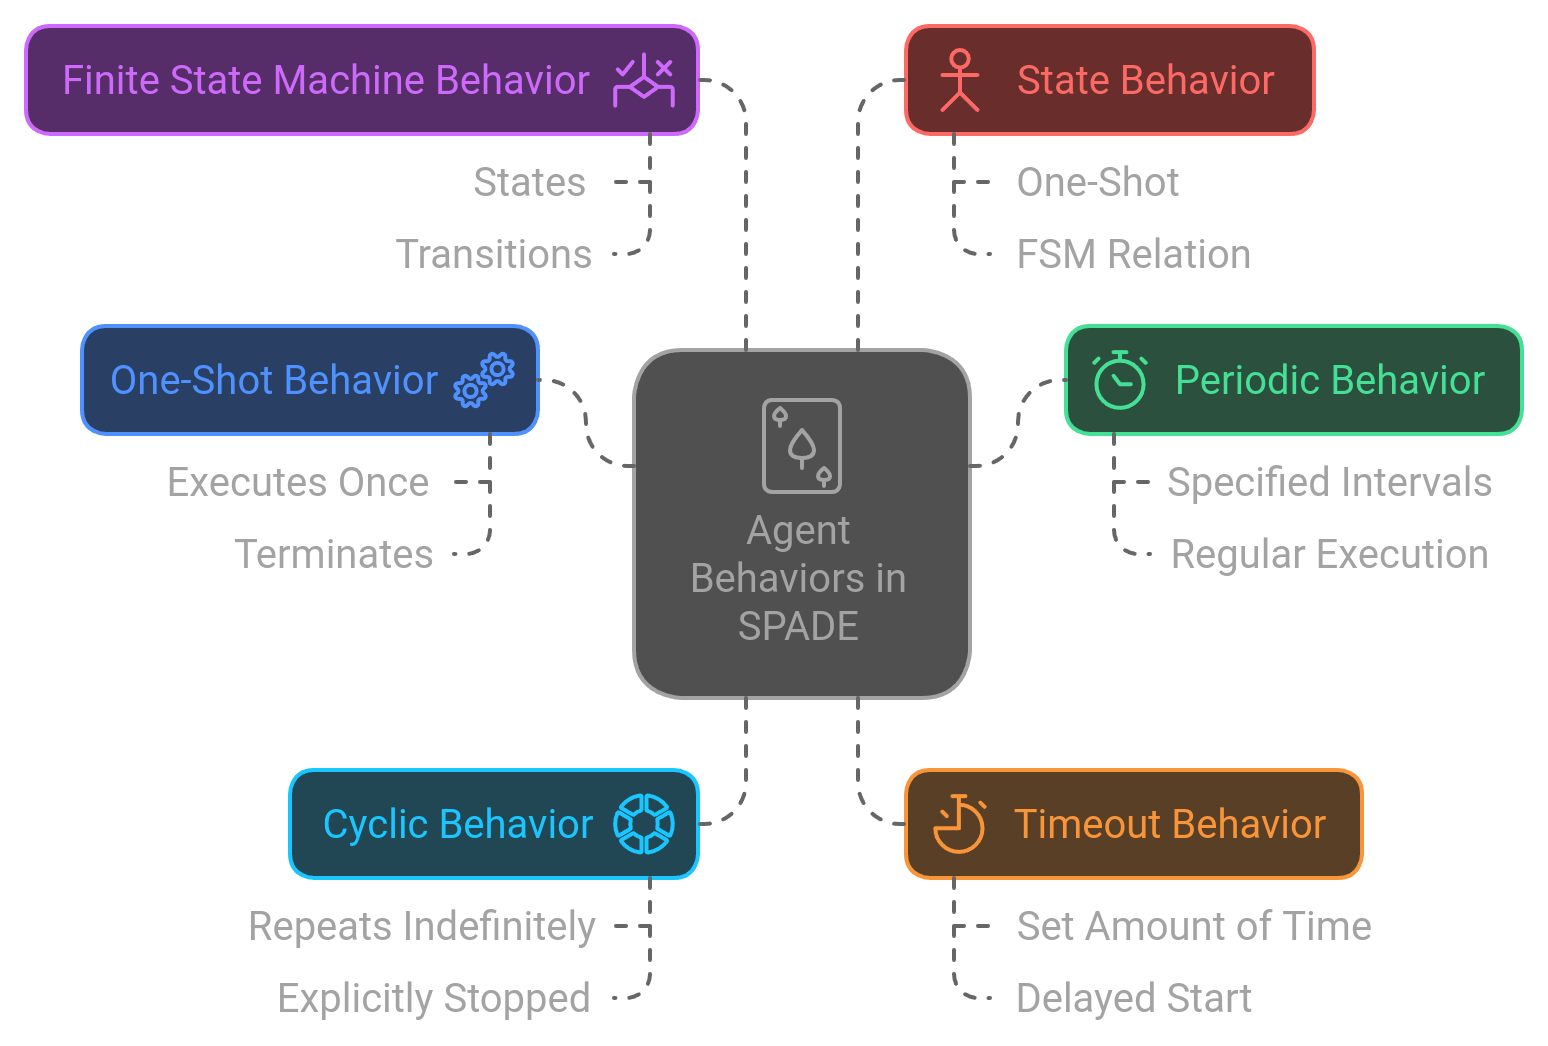
\includegraphics{Documents/241119 DSC Europe/Figures/Agent behaviours in SPADE dark.png}
    }{Different types of agent behaviours in \ac{SPADE}}{agent behaviours spade}
\end{frame}

\begin{frame}{\insertsection}
    \customFigure[0.45]{
        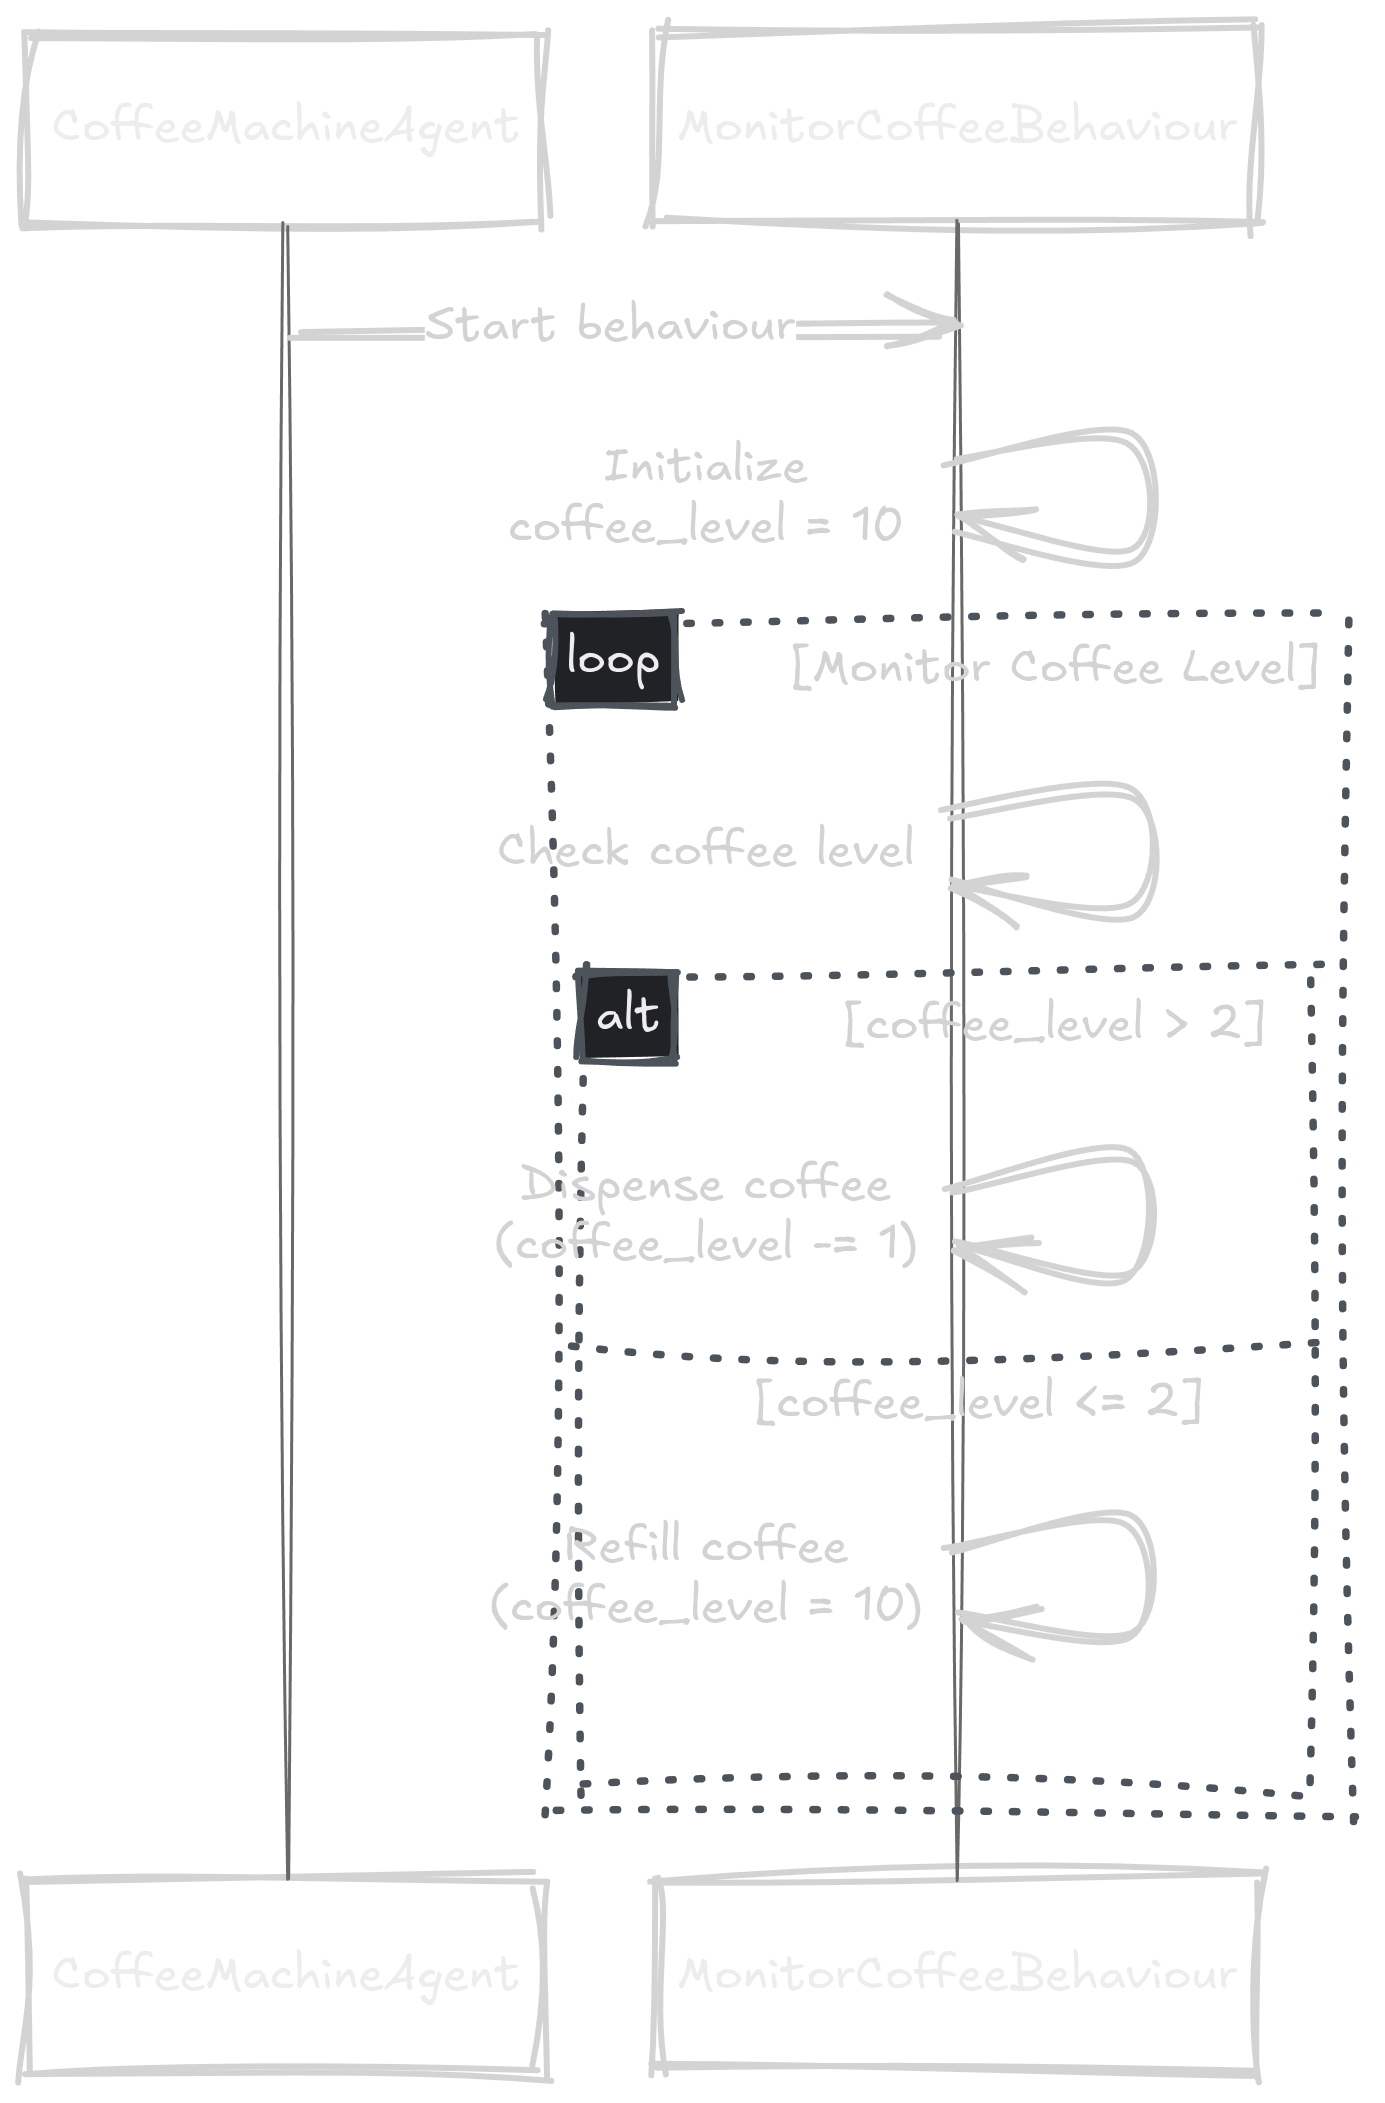
\includegraphics{Documents/241119 DSC Europe/Figures/agent coffee machine white.png}
    }{Visual representation of a simple coffee machine agent}{agent example coffee machine}
\end{frame}

\activityFrame{\mintedInline{agent coffee.py}}{https://github.com/AILab-FOI/MAGO/blob/main/Documents/241119\%20DSC\%20Europe/Implementation/agent\%20coffee.py}



\begin{frame}[fragile]{\insertsection: \insertsubsection}
    \begin{listing}
    \mintedFilePythonBlack[firstline=7, lastline=30]{Documents/241119 DSC Europe/Implementation/agent coffee.py}
    \caption{The coffee machine agent with a single behaviour}
    \end{listing}
\end{frame}



\begin{frame}{\insertsection}
    \customFigure[1]{
        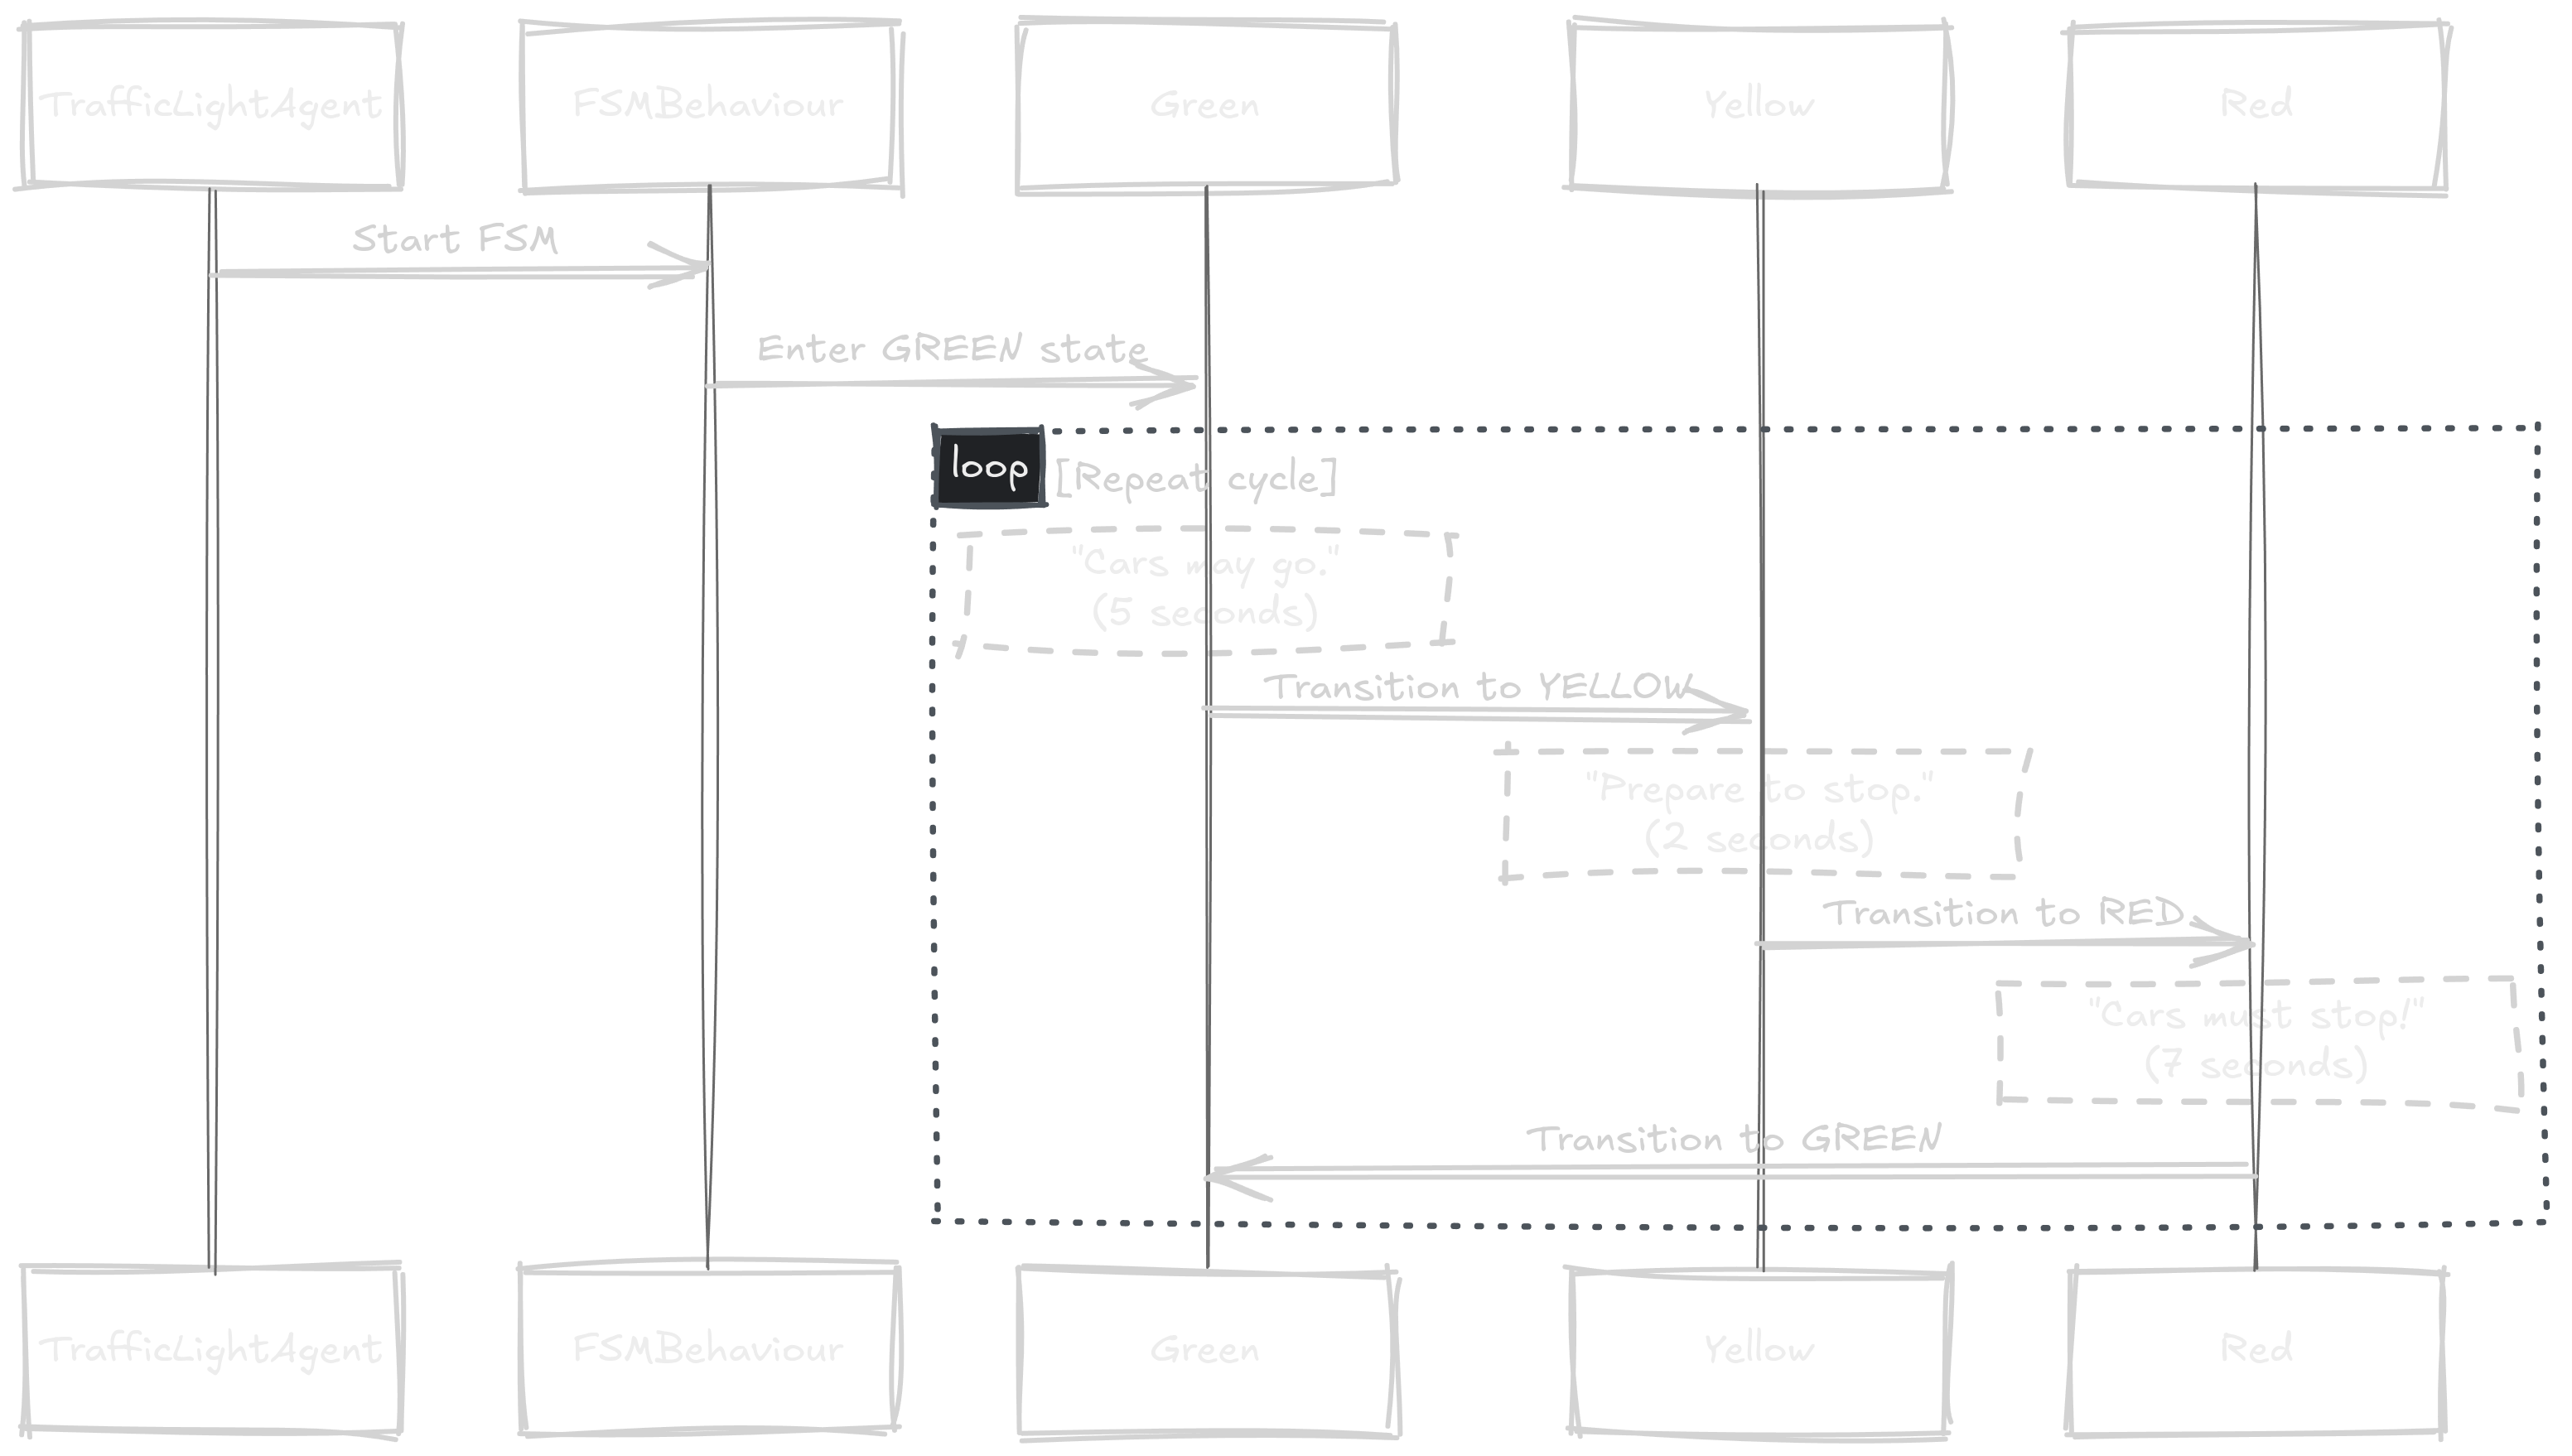
\includegraphics{Documents/241119 DSC Europe/Figures/example traffic light.png}
    }{Visual representation of a traffic light agent with a finite state machine behaviour}{agent example traffic light}
\end{frame}

\activityFrame{\mintedInline{agent traffic light.py}}{https://github.com/AILab-FOI/MAGO/blob/main/Documents/241119\%20DSC\%20Europe/Implementation/agent\%20traffic\%20light.py}

\begin{frame}[fragile]{\insertsection}
    \begingroup
    \setlength{\columnsep}{3em}
    \begin{multicols}{2}
        \begin{listing}
        \mintedFilePythonBlack[firstline=11, lastline=31]{Documents/241119 DSC Europe/Implementation/agent traffic light.py}
        \end{listing}

        \columnbreak
        
        \begin{listing}
        \mintedFilePythonBlack[firstline=34,lastline=50]{Documents/241119 DSC Europe/Implementation/agent traffic light.py}
        \caption{Traffic light agent with finite state machine behaviour}
        \end{listing}
    \end{multicols}
    \endgroup
\end{frame}



\begin{frame}{\insertsection}
    \customFigure[0.7]{
        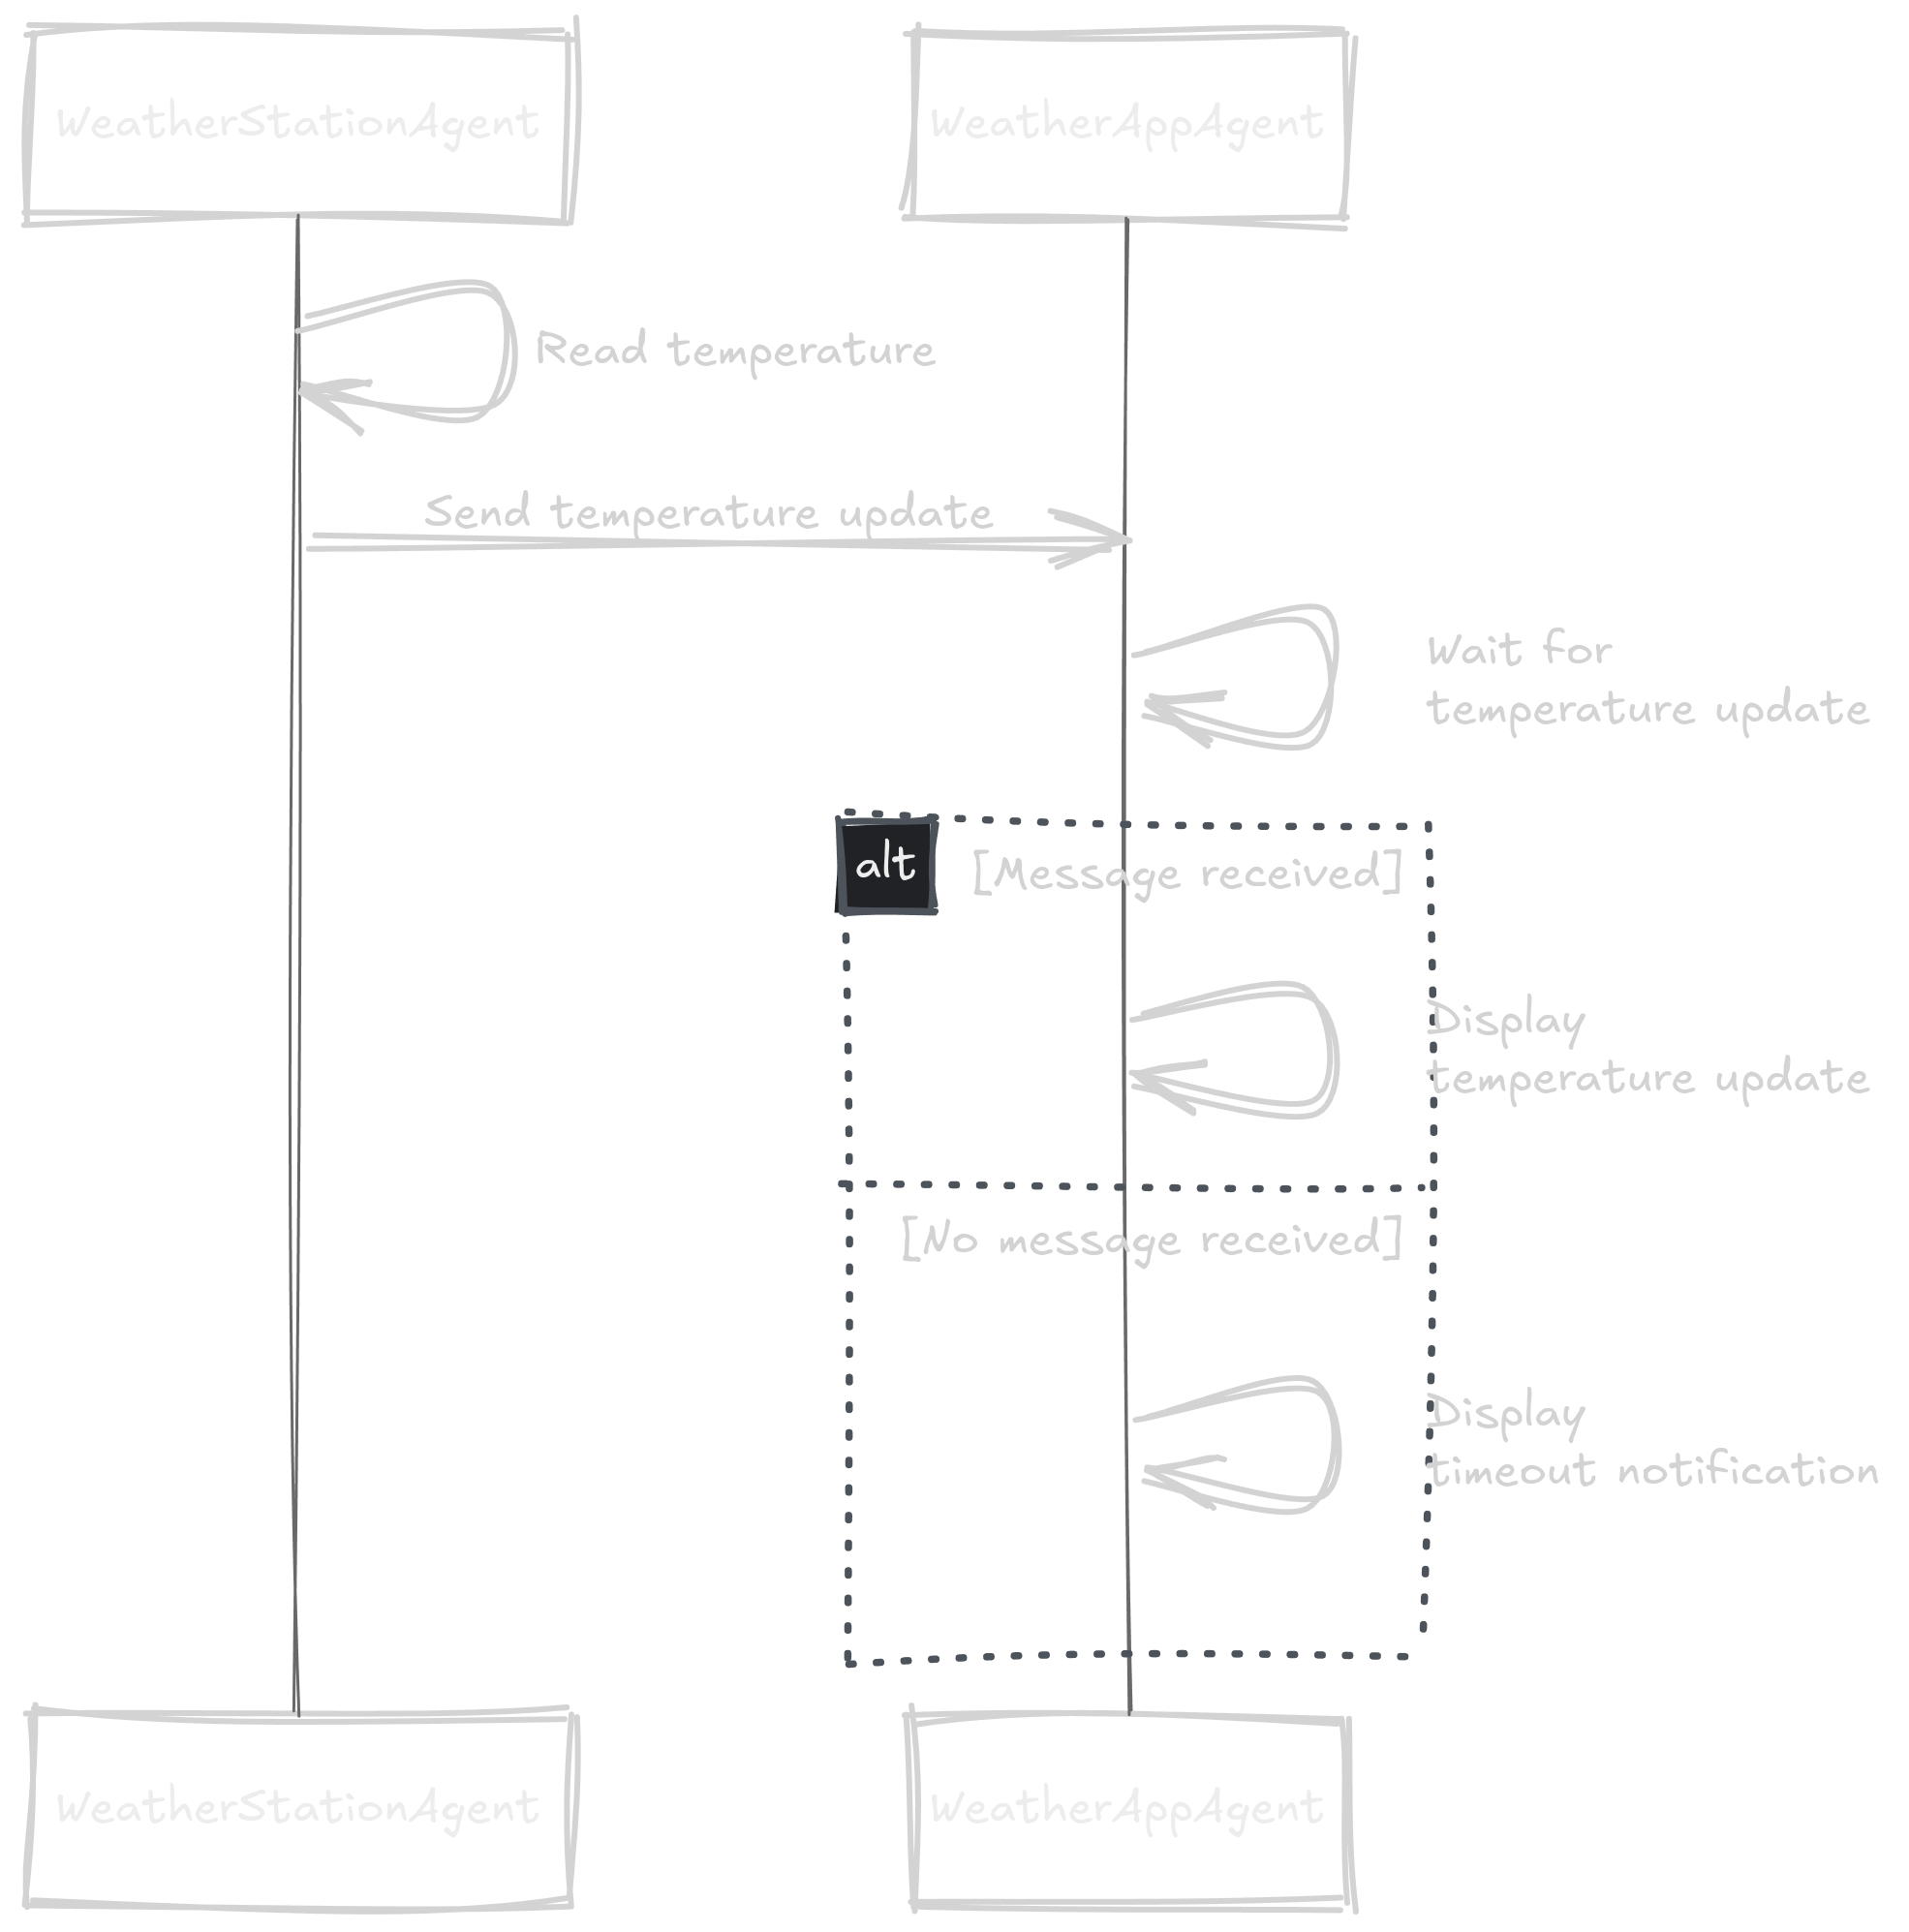
\includegraphics{Documents/241119 DSC Europe/Figures/weather agent example.png}
    }{Visual representation of two communicating agents}{agent example weather communication}
\end{frame}

\activityFrame{\mintedInline{agent weather.py}}{https://github.com/AILab-FOI/MAGO/blob/main/Documents/241119\%20DSC\%20Europe/Implementation/agent\%20weather.py}

\begin{frame}[fragile]{\insertsection}
    \begingroup
    \setlength{\columnsep}{3em}
    \begin{multicols}{2}
        \begin{listing}
        \mintedFilePythonBlack[firstline=9, lastline=24]{Documents/241119 DSC Europe/Implementation/agent weather.py}
        \end{listing}

        \columnbreak
        
        \begin{listing}
        \mintedFilePythonBlack[firstline=27,lastline=43]{Documents/241119 DSC Europe/Implementation/agent weather.py}
        \caption{Agent communication example}
        \end{listing}
    \end{multicols}
    \endgroup
\end{frame}